\section{Kartendarstellungen}
\label{sec:2}
 \subsection{Azimuthale äquidistante Projektion}
\label{sec:azimuequi}
Bei dieser Projektion ist die kürzeste Entfernung vom Mittelpunkt der Karte zu einem beliebigen anderen Punkt eine gerade Linie. Das bedeutet, dass alle Punkte, die auf einem Kreis um den Kartenmittelpunkt liegen, äquidistant sind.\\
Nachteil:\newline
Die Gebiete die auf der anderen Seite der Welt liegen, werden sehr verzehrt dargestellt. Daher ist diese Projektion für Weltkarten 
eher ungeeignet.\\
\begin{figure}[hbtp]
\centering
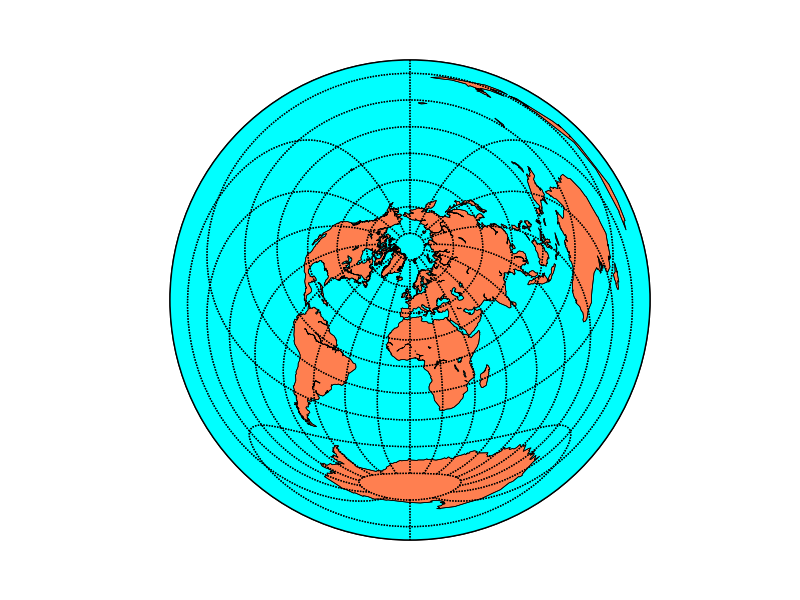
\includegraphics[scale=0.4,origin=c]{/Users/student/seminar/Kartendarstellungen/seminar/aziequi} \\
\caption{Azimuthale äquidistante Projektion}
\end{figure}
\clearpage
\subsection{Gnomonische Projektion}
\label{sec:gnomic}
In der gnomonischen Projektion werden alle Längenkreise als gerade Linien dargestellt.
Das Besondere der gnomonischen Projektion ist das der Projektionspunkt im Mittelpunkt der Erde liegt.
Da hier von Innen nach Außen projiziert wird, nimmt die Verzerrung mit der Entfernung vom Kartenmittelpunkt zu. Die gnomonische Projektion ist keine globale Projektion.\\

\begin{figure}[hbtp]
\centering
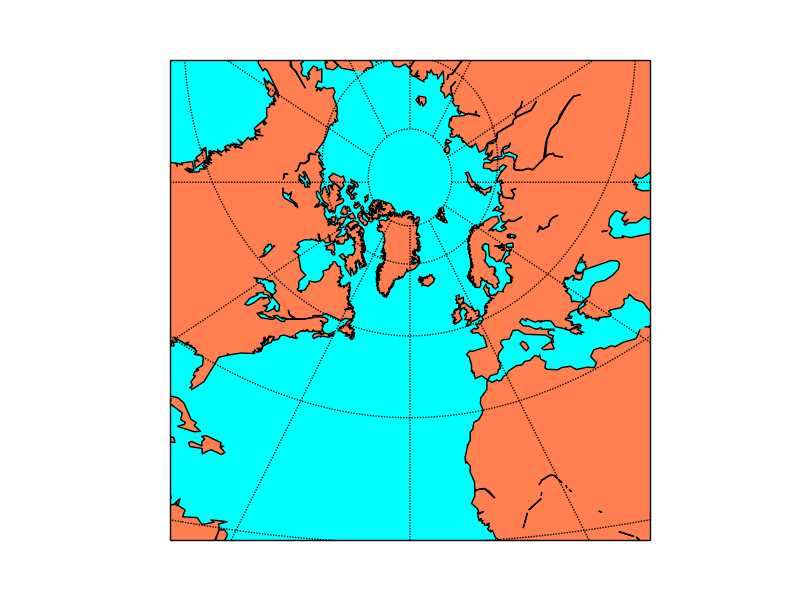
\includegraphics[scale=0.5,origin=c]{/Users/student/seminar/Kartendarstellungen/seminar/gnom} \caption{Gnomonische Projektion}
\end{figure}
\newpage 
\subsection{Orthographic Projection}
\label{sec:2.3}

\subsection{Geostationäre Projektion}
\label{sec:geostat}
In der geostationären Projektion wird die Erde aus der Perspektive eines geostationären Satelliten.
Vorteil:\newline \begin{itemize}
                  \item Wenn die Position des Satelliten bekannt ist, kann man dessen
                  Bilder als Hintergrund verwenden (siehe \ref{bilder})
                 \end{itemize}

Nachteil:\newline \begin{itemize}
                  \item Die andere Seite der Erde wird nicht dargestellt.\\
                  \item Entfernungen zwischen 2 Punkten werden auf Kreisbögen gemessen.\\
                  \item Der Satellit muss über dem Äquator sein.
                 \end{itemize}
\begin{figure}[hbtp]
\centering
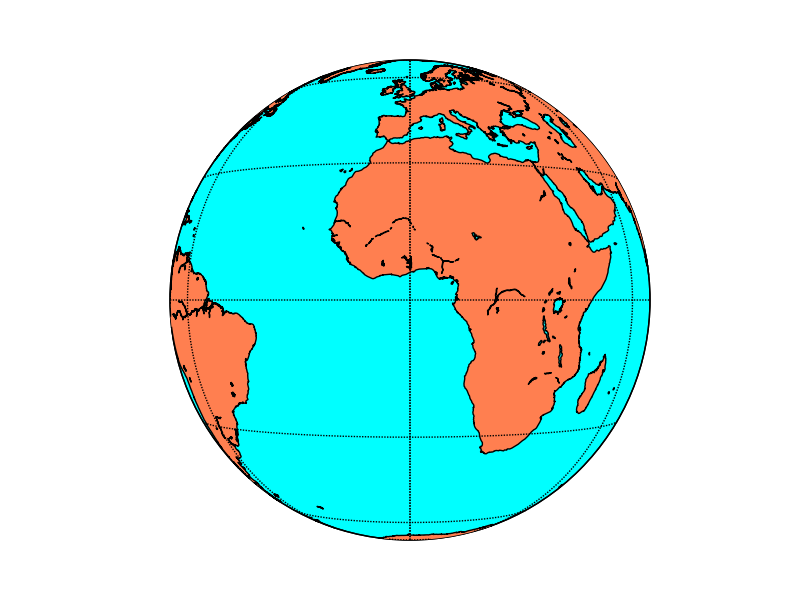
\includegraphics[scale=0.5,origin=c]{/Users/student/seminar/Kartendarstellungen/seminar/geos} \caption{Geostationäre Projektion}
\end{figure}
\newpage 
\subsection{Near-Sided perspektivische Projektion}
\label{sec:nearsideperspective}
Die Near Sided Perspective zeigt die Erde aus der Sicht eines Satelliten. Also ist es im Prinzip das selbe
wie die geostationäre Projektion.
\subsection{Mollweide Projection}
\label{sec:Mollweiden}
Bei der Mollweiden Projektion wird die Erde als Oval dargestellt. Die Mollweiden Projektion ist flächentreu.
Der Äquator und der Nullmeridian werden bei der Mollweiden Projektion maßstabsgetreu wieder gegeben.
Breitenkreise werden bei der Mollweiden Projektion als Geraden dargestellt. Die Längenkreise sind als Ellipsen dargestellt.
\subsection{Hammer Projektion}
\label{sec:Hammer}
Die Hammer Projektion ist wie die Mollweiden Projektion eine flächentreue Projektion.
Bei der Hammer Projektion wird die Erden ebenfalls als Oval dargestellt. Allerdings werden die Breitenkreise im Gegensatz zur Mollweiden Projektion als Ellipsen dargestellt, dadurch ist die Verzerrung an den Rändern nicht so stark. Nachteil bei dieser Art der Darstellung ist, dass die Erde an den Polen gestaucht wird.
\subsection{Robinson Projektion}
\label{sec:robinson}
Die Robinson Projektion ist eine globale Projektion. Die Erde wird hier annähernd Oval dargestellt. Die Pole werden allerdings in dieser Darstellung nicht abgedeckt. Breitenkreise werden in der Robinson Projektion als Geraden dargestellt. Bei dieser Darstellung wurden die Verzerrungen reduziert. Nachteil der Robinson Projektion ist das die Pole nicht erfasst werden.\\

\begin{figure}[hbtp]
\centering
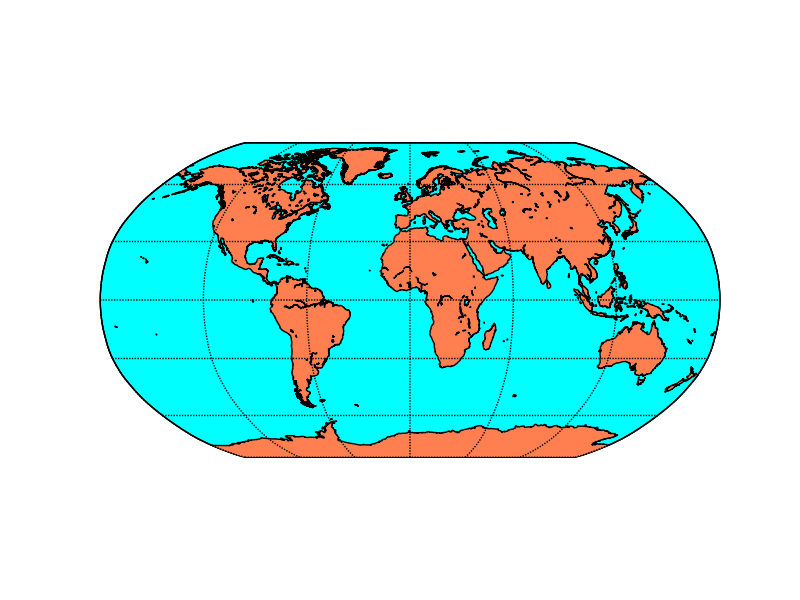
\includegraphics[scale=0.5,origin=c]{/Users/student/seminar/Kartendarstellungen/seminar/robin} \caption{Robinson Projektion}
\end{figure}
\newpage 
\subsection{Eckert 4 Projektion}
\label{sec:eckert4}
Die Eckert 4 Projektion ist sehr ähnlich wie die Robinson Projektion, allerdings ist Sie flächentreu. Deshalb ist die Darstellung an den Polen gestaucht. Die Erde wird wie auf einem Reifen dargestellt. Die Seitenränder sind in dieser Projektion Halbkreise.\newline
Formel:\newline

\begin{eqnarray*}
\mathcal{X}  & = & \frac{2}{\sqrt{4\pi +\pi ^2}}{\cal R}(\lambda -\lambda _0\footnote{Der zentrale Längenkreis} ) (1+\cos \theta)\\
\mathcal{Y}  & = & 2\sqrt{\dfrac{\pi }{4+\pi }}\cal R \sin \theta \\
\theta +\sin \theta \cos \theta +2\sin \theta & = &\left( 2+\frac{\pi }{2} \right) \sin \varphi
\end{eqnarray*}

\begin{figure}[hbtp]
\centering
 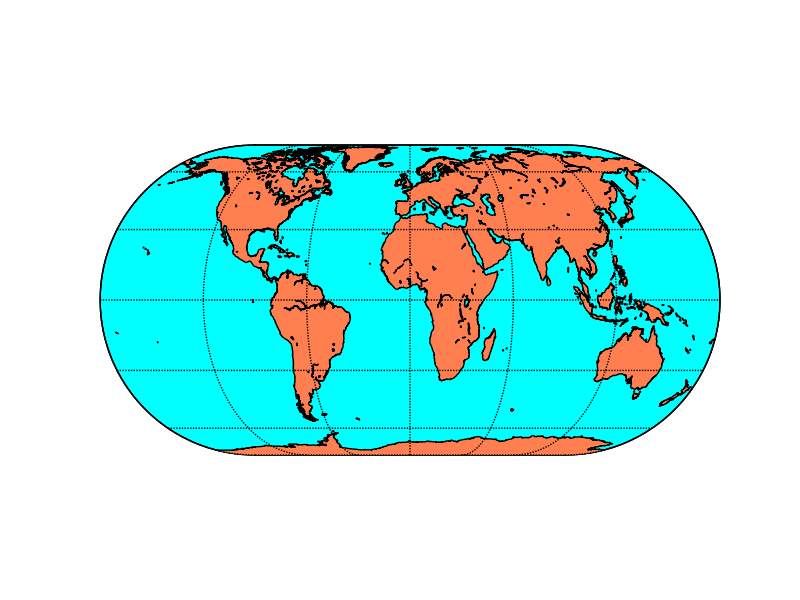
\includegraphics[scale=0.5,origin=c]{/Users/student/seminar/Kartendarstellungen/seminar/eck4} 
\caption{Eckert 4 Projektion}
\end{figure}
\newpage 
\subsection{Kavrayskiy 7 Projektion}
\label{sec:kravrayskiy}
Die Kavrayskiy 7 Projektion ist der Robinson Projektion sehr ähnlich. Sie stellt die Erde wieder annähernd oval dar. Die Breitenkreise werden in dieser Projektion als Geraden dargestellt. Diese Projektion stellt einen Kompromiss zwischen winkeltreuen und flächentreuen Projektionen dar.
\subsection{McBryde-Thomas Projektion}
\label{sec:mcbryde-thomas}
Diese Projektion ist eine flächentreue Darstellung der Erde. Die Breitenkreise werden als Geraden dargestellt. Die Längenkreise werden als Bögen dargestellt. Dabei haben die Längenkreise, auf einem Breitenkreis, immer den gleichen Abstand zueinander. Die Breitenkreise hingegen stehen immer näher je näher man den Polen kommt. Die Pole sind auf ein drittel des Äquators gestreckt. Der Nullmeridian ist in dieser Projektion 0,45 mal so lang wie der Äquator.

%Grapfik
\subsection{Sinusoidale Projektion}
\label{sec:sinusodial}
Die sinusoidale Projektion ist eine flächentreue Projektion. Auch in dieser Projektion werden die Breitenkreise als Geraden dargestellt. Das besondere an der sinusoidalen Projektion ist das die Länge der Breitenkreise relational zu $\cos\varphi$ ist, dies führt zu einer starken Verzerrung außerhalb der Mitte.\\
Vorteil der sinusoidalen Projektion:\\
\begin{itemize}
\item Die Projektion ist einfach zu berechnen.
\end{itemize}
Nachteil der sinusoidalen Projektion:\\
\begin{itemize}
\item Die Projektion ist nicht sehr anschaulich.
\end{itemize}
Formel:\\
\begin{eqnarray}
\mathcal {X} & = &\cal{R}\cdot(\lambda - \lambda _0)\cdot \cos \varphi \\
\mathcal{Y} & = &\cal{R} \cdot \varphi
\end{eqnarray}

\subsection{Äquidistante Zylinder Projektion}
\label{sec:aequizylinder} 
Die äquidistante Zylinder Projektion ist die einfachste Projektion. Sie stellt die Erde einfach in Längen- und Breitengrad dar. Dabei entsteht ein gleichmäßiges Gitterraster. Die Projektion ist weder winkel- noch flächentreu, das heißt, dass die Verzerrung mit der Entfernung vom Mittelpunkt der Karte zunimmt.\\ 
Vorteil der äquidistanten Zylinder Projektion:
\begin{itemize}
\item Die Projektion ist sehr einfach zu berechnen.
\end{itemize}
Nachteil der äquidistanten Zylinder Projektion:\\
\begin{itemize}
\item Die Verzerrungen wirken sowohl auf die Fläche als auch auf die Abstände aus.
\end{itemize}

Formel:\\
\begin{eqnarray}
\cal{X} & = & \lambda\\
\cal{Y} & = & \varphi
\end{eqnarray}
\subsection{Cassini Projektion}
\label{sec:cassini}
Bei der Cassini Projektion wird die Erde zuerst gedreht, sodass der Äquator zum Nullmeridian wird.
Danach wird dann eine äquidistante Zylinder Projektion angewendet. \\

\begin{figure}[hbtp]
\centering
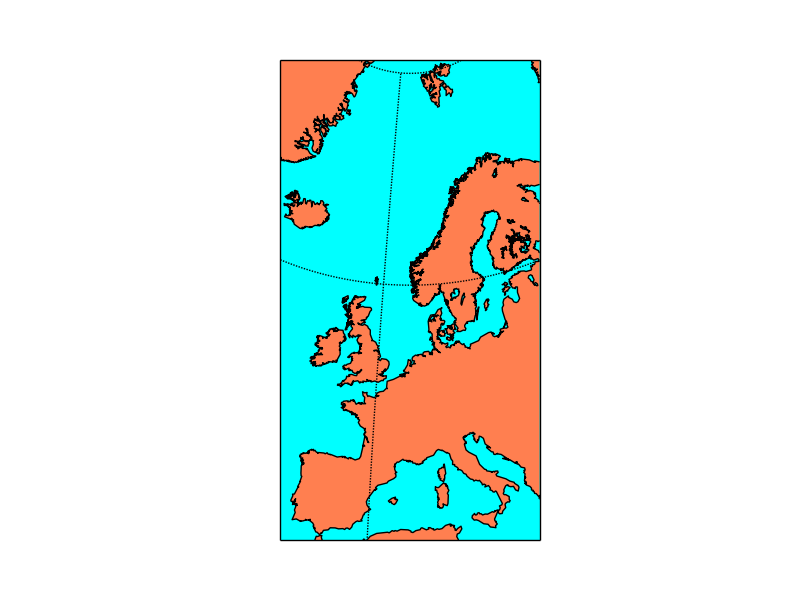
\includegraphics[scale=0.5,origin=c]{/Users/student/seminar/Kartendarstellungen/seminar/cass} \caption{Cassini Projektion}
\end{figure}
\newpage 
\subsection{Mercatorprojektion}
\label{sec:mercator} 
Die Mercatorprojektion ist eine winkeltreue Zylinderprojektion. Sie erreicht dabei nie Pole.
Die Längengrade verlaufen in dieser Projektion parallel und haben den gleichen Abstand zueinander.
Die Breitengrade sind ebenfalls parallel zueinander haben aber unterschiedliche Abstände.
Die Verzerrung nimmt mit Polnähe zu, das heißt, dass die Karte zu den Polen hin gestreckt wird.\\

\begin{figure}[hbtp]
\centering
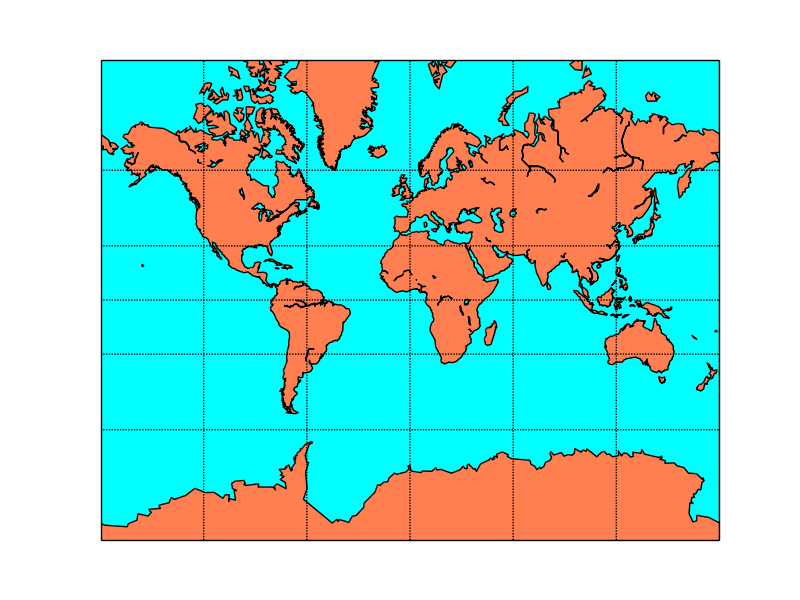
\includegraphics[scale=0.5,origin=c]{/Users/student/seminar/Kartendarstellungen/seminar/merc} \caption{Mercatorprojektion}
\end{figure}
\newpage 
\subsection{Transversale Mercatorprojektion}
\label{sec:transmercator}
Bei der transversalen  Mercatorprojektion wird der Globus zuerst um 90° gedreht, so das der 0 Meridian zu Äquator wird. Danach wird eine normale Mercatorprojektion erstellt.
\subsection{Oblique Mercator Projection}
\label{sec:2.17}
\subsection{Polykonische Projektion}
\label{sec:polikonisch}
Die polikonische Projektion ist eine globale Projektion. Hierbei werden auf dem zentralen Meridian unendlich viele Kegel aufgebaut. Dabei entstehen nicht konzentrische Breitenkreise. Die Projektion geht an den Polen auseinander. Die Verzerrung der Fläche nimmt mit der Entfernung vom zentralen Meridian der Karte zu. Die Winkel sind lokal entlang des zentralen Längengrades genau, sonst sind sie verzerrt.
\subsection{Miller Zylinderprojektion}
\label{sec:miller}
Die Miller Zylinderprojektion ist eine globale Projektion. Sie ist der Mercatorprojektion sehr ähnlich.
Allerdings ist hier die Verzerrung an den Polen anders. Die Pole werden nicht mehr so stark gesteckt, dafür ist die Miller-Projektion nicht winkeltreu. Dafür reicht die Miller Zylinderprojektion bis an die Pole. \\

\begin{figure}[hbtp]
\centering
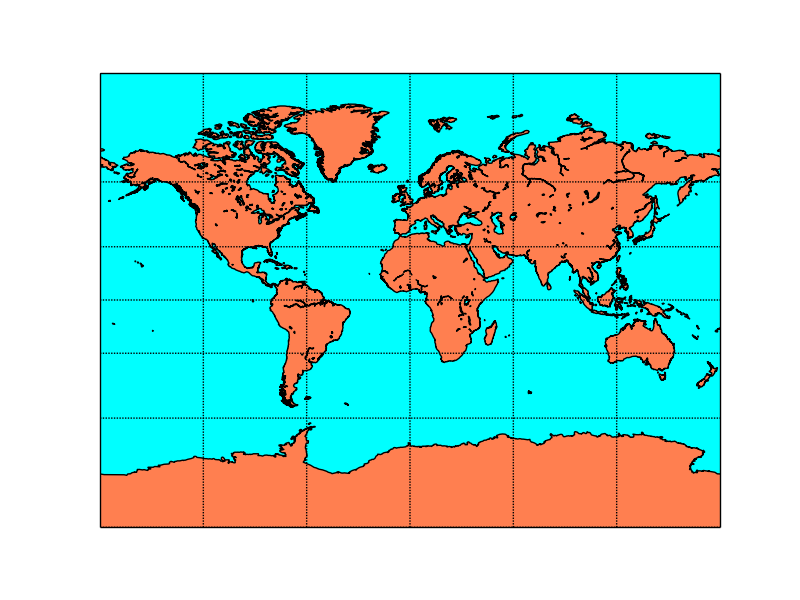
\includegraphics[scale=0.5,origin=c]{/Users/student/seminar/Kartendarstellungen/seminar/mill} \caption{Miller Zylinderprojektion}
\end{figure}
\newpage 
\subsection{Stereographische Gall Projektion}
\label{sec:stereogall} 
Die stereographische Gall Projektion ist eine globale Zylinderprojektion. Die Gall Projektion hat zwei Standartparallelen bei 45$ ^\circ $N und 45$^\circ $S. Die Verzerrung der Fläche und Winkel nimmt mit Abstand zu den Standartparallelen zu. Die Verzerrung ist allgemein an den Polen sehr stark. \\

\begin{figure}[hbtp]
\centering
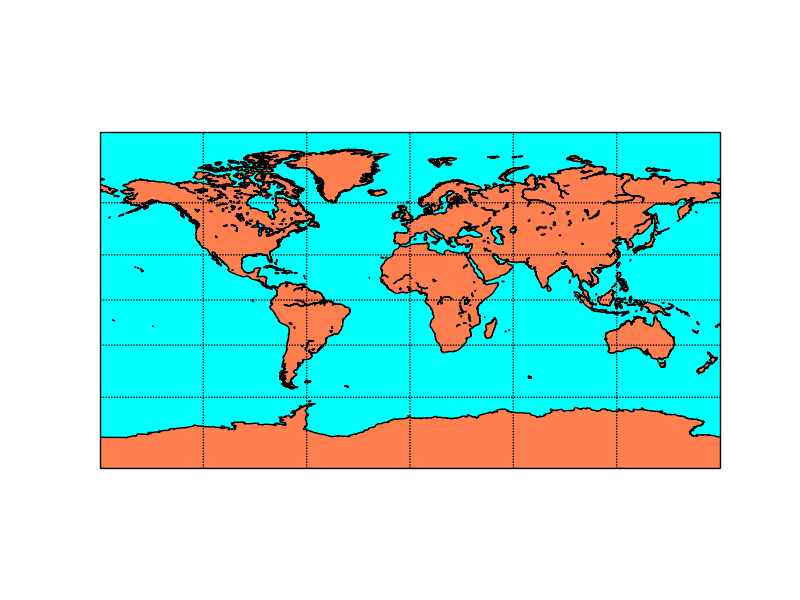
\includegraphics[scale=0.5,origin=c]{/Users/student/seminar/Kartendarstellungen/seminar/gall} \caption{Stereographische Gall Projektion}
\end{figure}
\newpage 
\subsection{Flächentreue Zylinderprojektion}
\label{sec:equareazyl}
Die flächentreue Zylinderprojektion ist eine flächentreue Zylinderprojektion wie es der Name bereits sagt. 
\subsection{ Winkeltreue Lambert Projektion}
\label{sec:lamwink}
Die winkeltreue Lambert Projektion ist winkeltreu. Die Längenkreise werden als Geraden dargestellt.
Die winkeltreue Lambert Projektion ist eine Kegelprojektion. 

Formel:\\
 \begin{eqnarray*}
 \mathcal{X}& = &\rho \sin ( n(\lambda -\lambda _0) )\\
 \mathcal{Y}& = &\rho _0-\rho \cos (n(\lambda - \lambda _0))\\
 \rho & = &F\cot ^n(\frac{1}{4}\pi + \frac{1}{2}\varphi)\\
 n& = &\dfrac{\ln (\cos \varphi _1 \sec \varphi _2)}{\ln (\tan (\frac{1}{4}\pi +\frac{1}{2}\varphi _2)\cot (\frac{1}{4}\pi + \frac{1}{2}\varphi _1))}\\
 F& = &\dfrac{\cos \varphi _1 \tan ^n(\frac{1}{4}\pi +\frac{1}{2}\varphi _1)}{n}
 \end{eqnarray*}\\
 
\begin{figure}[hbtp]
\centering
 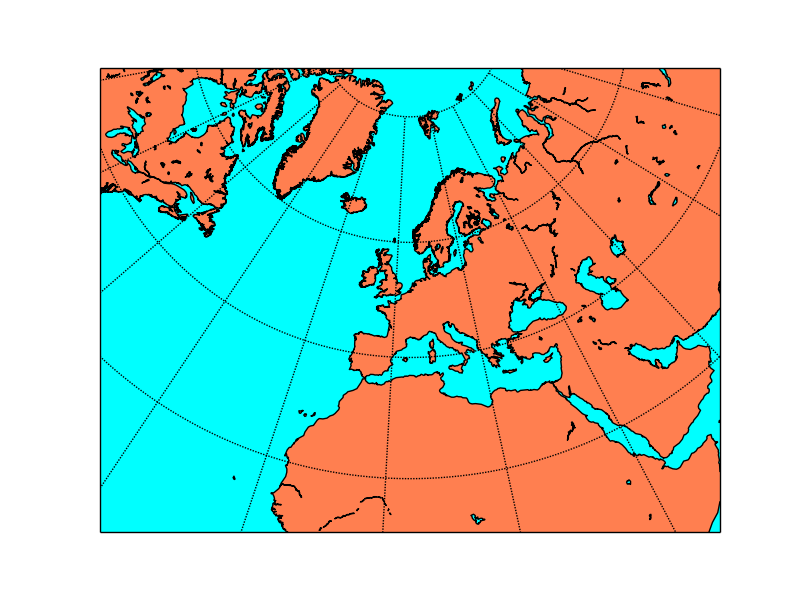
\includegraphics[scale=0.5,origin=c]{/Users/student/seminar/Kartendarstellungen/seminar/lcc} \caption{Winkeltreue Lambert-Projektion}
\end{figure}
\newpage 
\subsection{Azimuthale Flächentreue Lambert-Projektion}
\label{sec:lamflach}
\subsection{Stereographic Projection}
\label{sec:2.24}
\subsection{Equidistant Conic Projection}
\label{sec:2.25}
\subsection{Albers Equal Area Projection}
\label{sec:2.26}
\subsection{Polar Stereographic Projection}
\label{sec:2.27}
\subsection{Polar Lambert Azimuthal Projection}
\label{sec:2.28}
\subsection{Polar Azimuthal Equidistant Projection}
\label{sec:2.29}
\subsection{van der Grinten Projection}
\label{sec:2.30}
